With the MFV assumption, the top and bottom
quark can play an important  role in the phenomenology.
The scalar and pseudoscalar mediator models predict not only
the monojet process described in Section~\ref{sec:monojet_scalar}, but also production of Dark Matter
in association with top (or bottom) pairs, as illustrated in Fig.~\ref{fig:TTbarPhi}. 
Dedicated searches including jets from heavy flavor quarks in the final state
can be designed for this signature. Another class of simplified models,  
which includes a Dark Matter interpretation among many others, and yields a single
top quark in the final state, is detailed in Appendix~\ref{sec:singletop}. 

\begin{figure}[htbp!]
\centering
\vspace{0.5\baselineskip}
  \unitlength=0.005\textwidth
  \begin{feynmandiagram}[modelTTbarMET]
    \fmfleft{i1,i2}
    \fmfright{o1,o4,o5,o3}
    \fmf{gluon}{i1,v1}
    \fmf{gluon}{i2,v2}
    \fmf{fermion}{o1,v1,v3,v2,o3}
    \fmf{scalar}{v3,v4}
    \fmf{fermion}{o5,v4,o4}
    \fmf{phantom,tension=0,label={$\phi/a$}}{v3,v4}    
    \fmflabel{\Large $g$}{i1}
    \fmflabel{\Large $g$}{i2}
    \fmflabel{\Large $t (b)$}{o1}
    \fmflabel{\Large $\bar t (\bar b)$}{o3}
    \fmflabel{\Large $\chi$}{o4}
    \fmflabel{\Large $\bar \chi$}{o5}    
  \end{feynmandiagram}
\vspace{0.5\baselineskip}
\caption{Representative Feynman
diagram showing the pair production of Dark Matter particles in
association with $t\bar t$ (or $b\bar b$).}
\label{fig:TTbarPhi}
\end{figure}

In addition to the $t\bar t$+DM models illustrated in Fig.~\ref{fig:TTbarPhi}, 
some theoretically motivated scenario (e.g. for high $tan\beta$ in 2HDM in the pMSSM) 
privilege the coupling of \spinzero mediators to down generation quarks.
This assumption motivates the study of final states involving $b$-quarks 
as a complementary search to the $t\bar
t$+DM models, to directly probe the $b$-quark coupling. 
An example of such a model can be found in Ref.~\cite{Buckley:2014fba}
and can be obtained by replacing top quarks with $b$ quarks in Fig.~\ref{fig:TTbarPhi}.
Note that, because of the kinematics features of $b$ quark production relative
to heavy $t$ quark production, a $b\bar b$+DM final state may only yield one
experimentally visible $b$ quark, leading to a mono-$b$ signature in a model that conserves $b$ flavor.

Dedicated implementations of these models for the work of this Forum are available at LO+PS accuracy,
even though the state of the art is set to improve on a timescale beyond that for early Run-2 DM searches
as detailed in Section~\ref{sec:TTBar_implementation}.
The studies in this Section have been produced using a leading order UFO model within \madgraph 2.2.2
~\cite{Alwall:2014hca,Alloul:2013bka,Degrande:2011ua} 
using \pythiaEight for the parton shower. 

\paragraph{Parameter scan}

The parameter scan for the dedicated $t\bar{t}$+\MET{} searches has been studied in detail to target the production 
mechanism of DM associated with heavy flavor quarks, and shares many details of the scan for the scalar model with a gluon radiation.
The benchmark points scanning the model parameters have been selected to ensure that the kinematic features of the 
parameter space are sufficiently represented. Detailed studies were performed to identify points in the \mdm, 
$m_{\phi,a}$, $\gDM$, $\gq$ (and $\Gamma_{\phi,a}$) parameter space that differ significantly from each other 
in terms of expected detector acceptance. Because missing transverse momentum is the key observable for searches, the 
mediator $p_{T}$ spectra is taken to represent the main kinematics of a model. Another consideration in determining the set 
of benchmarks is to focus on the parameter space where we expect the searches to be sensitive during the 2015 LHC run. 
Based on a projected integrated luminosity of $30\,{\rm fb}^{-1}$ expected for 2015, we disregard model points with a 
cross section times branching ratio smaller than $0.1\,{\rm fb}$, corresponding to a minimum of one expected event 
assuming a 0.1\% efficiency times acceptance. 

The kinematics is most dependent on the masses \mdm and $m_{\phi,a}$. Figure~\ref{fig:scanPhi} 
and~\ref{fig:scanPhiPseudo} show typical dependencies for scalar and pseudoscalar couplings respectively.
Typically, the mediator $p_T$ spectrum broadens with larger $m_{\phi,a}$. 
The kinematics are also different between on-shell ($\mMed>2\mdm$) and off-shell ($\mMed<2\mdm$) mediators as discussed in Section~\ref{sec:monojet_scalar}. 
Furthermore, the kinematic differences in the \MET{} spectrum between scalar and pseudoscalar are larger for light mediator 
masses with respect to heavier mediators. It is therefore important to  
choose benchmark points covering on-shell and off-shell mediators with sufficient granularity, including the
transition region between on-shell and off-shell mediators. %, as inFig.~\ref{fig:scanPhidiag}. 

\begin{figure}[!ht]
  \begin{center}
    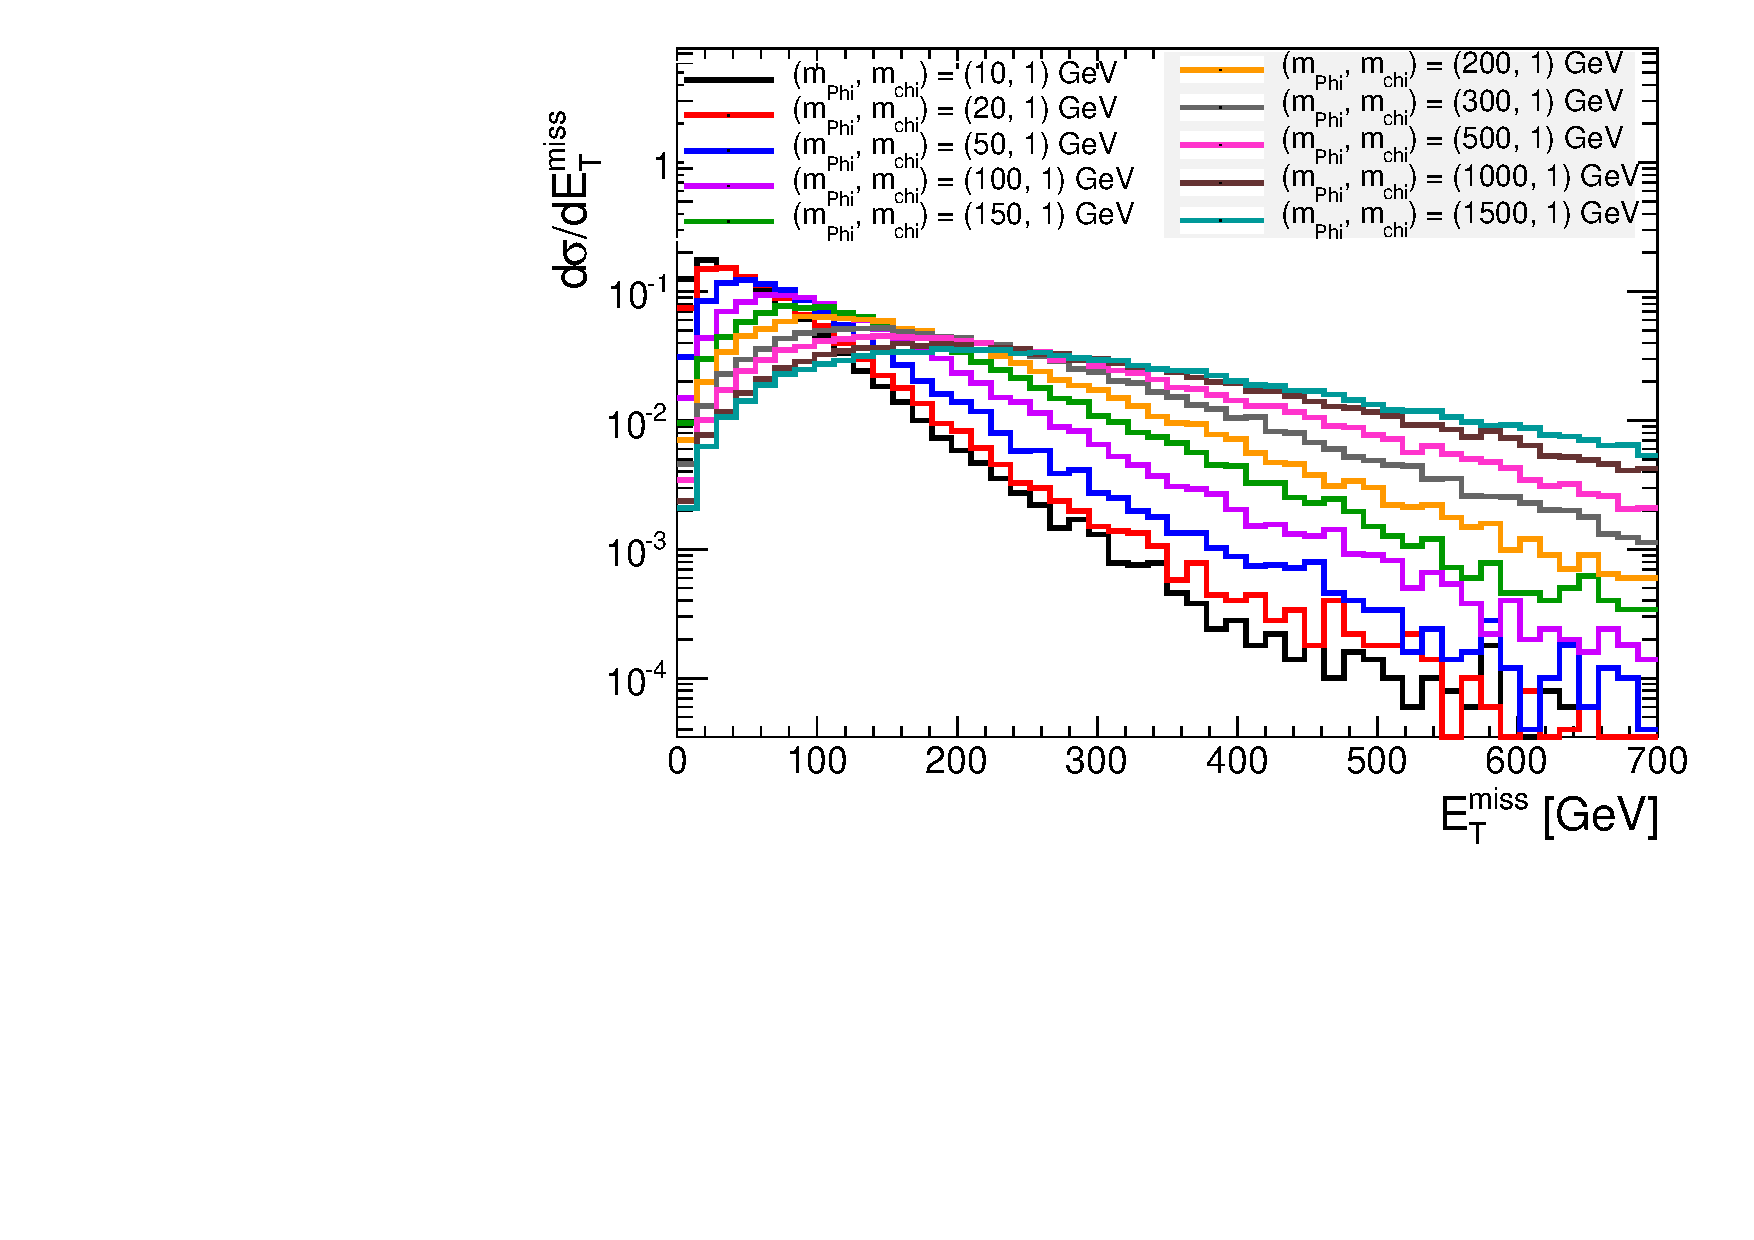
\includegraphics[width=0.95\textwidth]{figures/ttbar/MEt_chi1.pdf}
    \caption{\label{fig:scanPhi} Example of the dependence of the kinematics on the scalar mediator mass in the $t\bar{t}$+\MET{} signature. The Dark Matter mass is fixed to be \mdm=$1 {\rm GeV}$.}
\end{center}
\end{figure}


\begin{figure}[!ht]
  \begin{center}
    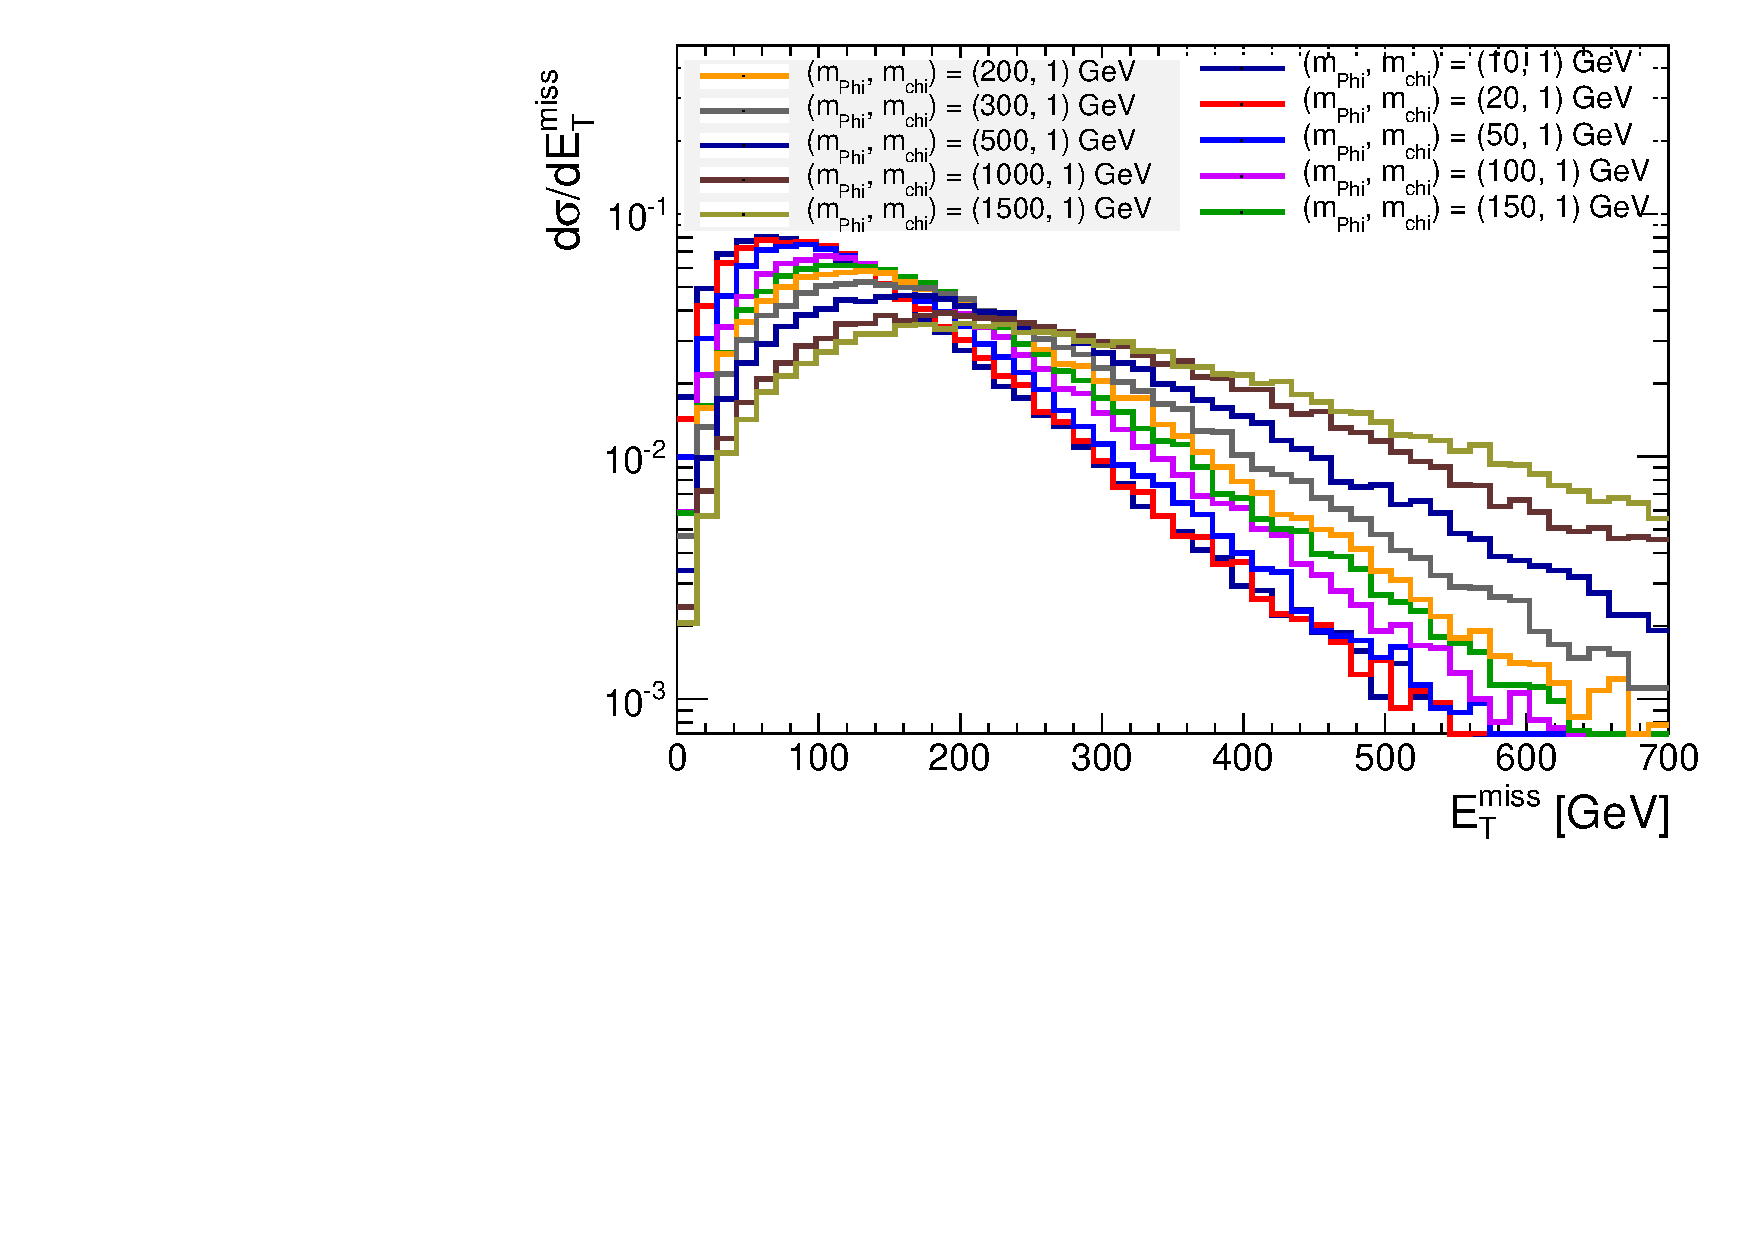
\includegraphics[width=0.95\textwidth]{figures/ttbar/MEt_chi1_pseudo.pdf}
    \caption{\label{fig:scanPhiPseudo} Example of the dependence of the kinematics on the pseudoscalar mediator mass in the $t\bar{t}$+\MET{}. The Dark Matter mass is fixed to be \mdm=$1 {\rm GeV}$. All figures concerning the $t\bar{t}$+\MET{}  signature have been produced using a leading order model within \madgraph 2.2.2, using \pythiaEight for the parton shower.}
\end{center}
\end{figure}

Typically only weak dependencies on couplings are observed (see Fig~\ref{fig:widthsmallscan}) where the variation with width of the integral over parton distributions is unimportant. As shown in Section~\ref{sub:parameter_scan_monojet}, for couplings $\sim O(1)$ the width is large enough that the $p_T$ of the mediator is determined mainly by the PDF. 

At large mediator masses ($\sim 1.5\,{\rm TeV}$) or very small couplings ($\sim 10^{-2}$), width effects are significant, but these regimes have production cross sections that are too small to be relevant for $30\,{\rm fb}^{-1}$ and are not studied here. However, with the full Run~2 dataset, such models may be within reach. 

\begin{figure}[!ht]
  \begin{center}
    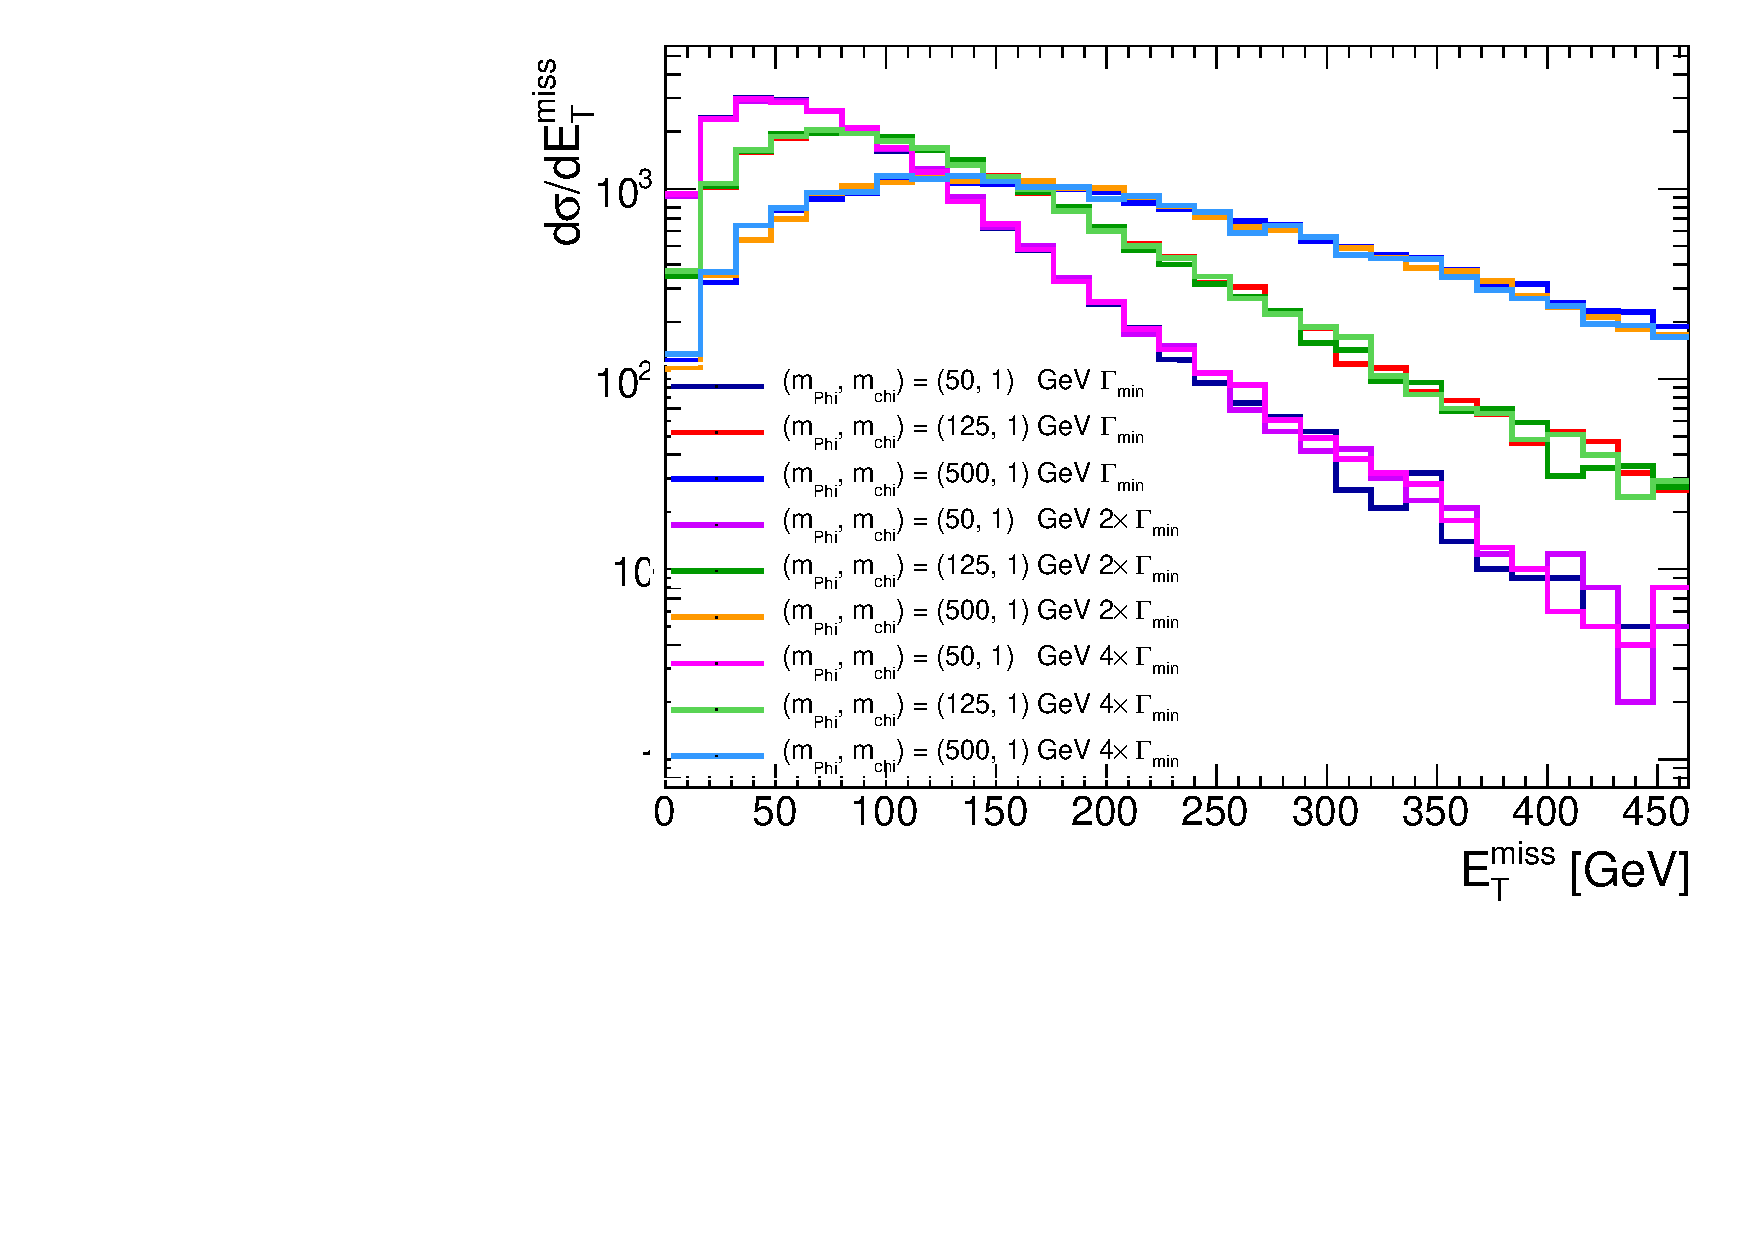
\includegraphics[width=0.95\textwidth]{figures/ttbar/MEt_smallwidth.pdf}
    \caption{\label{fig:widthsmallscan} Study of the dependence of kinematics on the width of a scalar mediator $t\bar{t}$+\MET{}. The width is increased up to four times the minimal width for each mediator and Dark Matter mass combination. 
    }
\end{center}
\end{figure}

Another case where the width can impact the kinematics is when $m_{\phi,a}$ is slightly larger than $2m_\chi$. Here, the width determines the relative contribution between on-shell and off-shell mediators. An example is given in Fig.~\ref{fig:widthlargescan}. As the minimal width choice pursued in this document is the most conservative one, this effect can be neglected in order to reduce the number of benchmark points to be generated. 

\begin{figure}[!ht]
  \begin{center}
    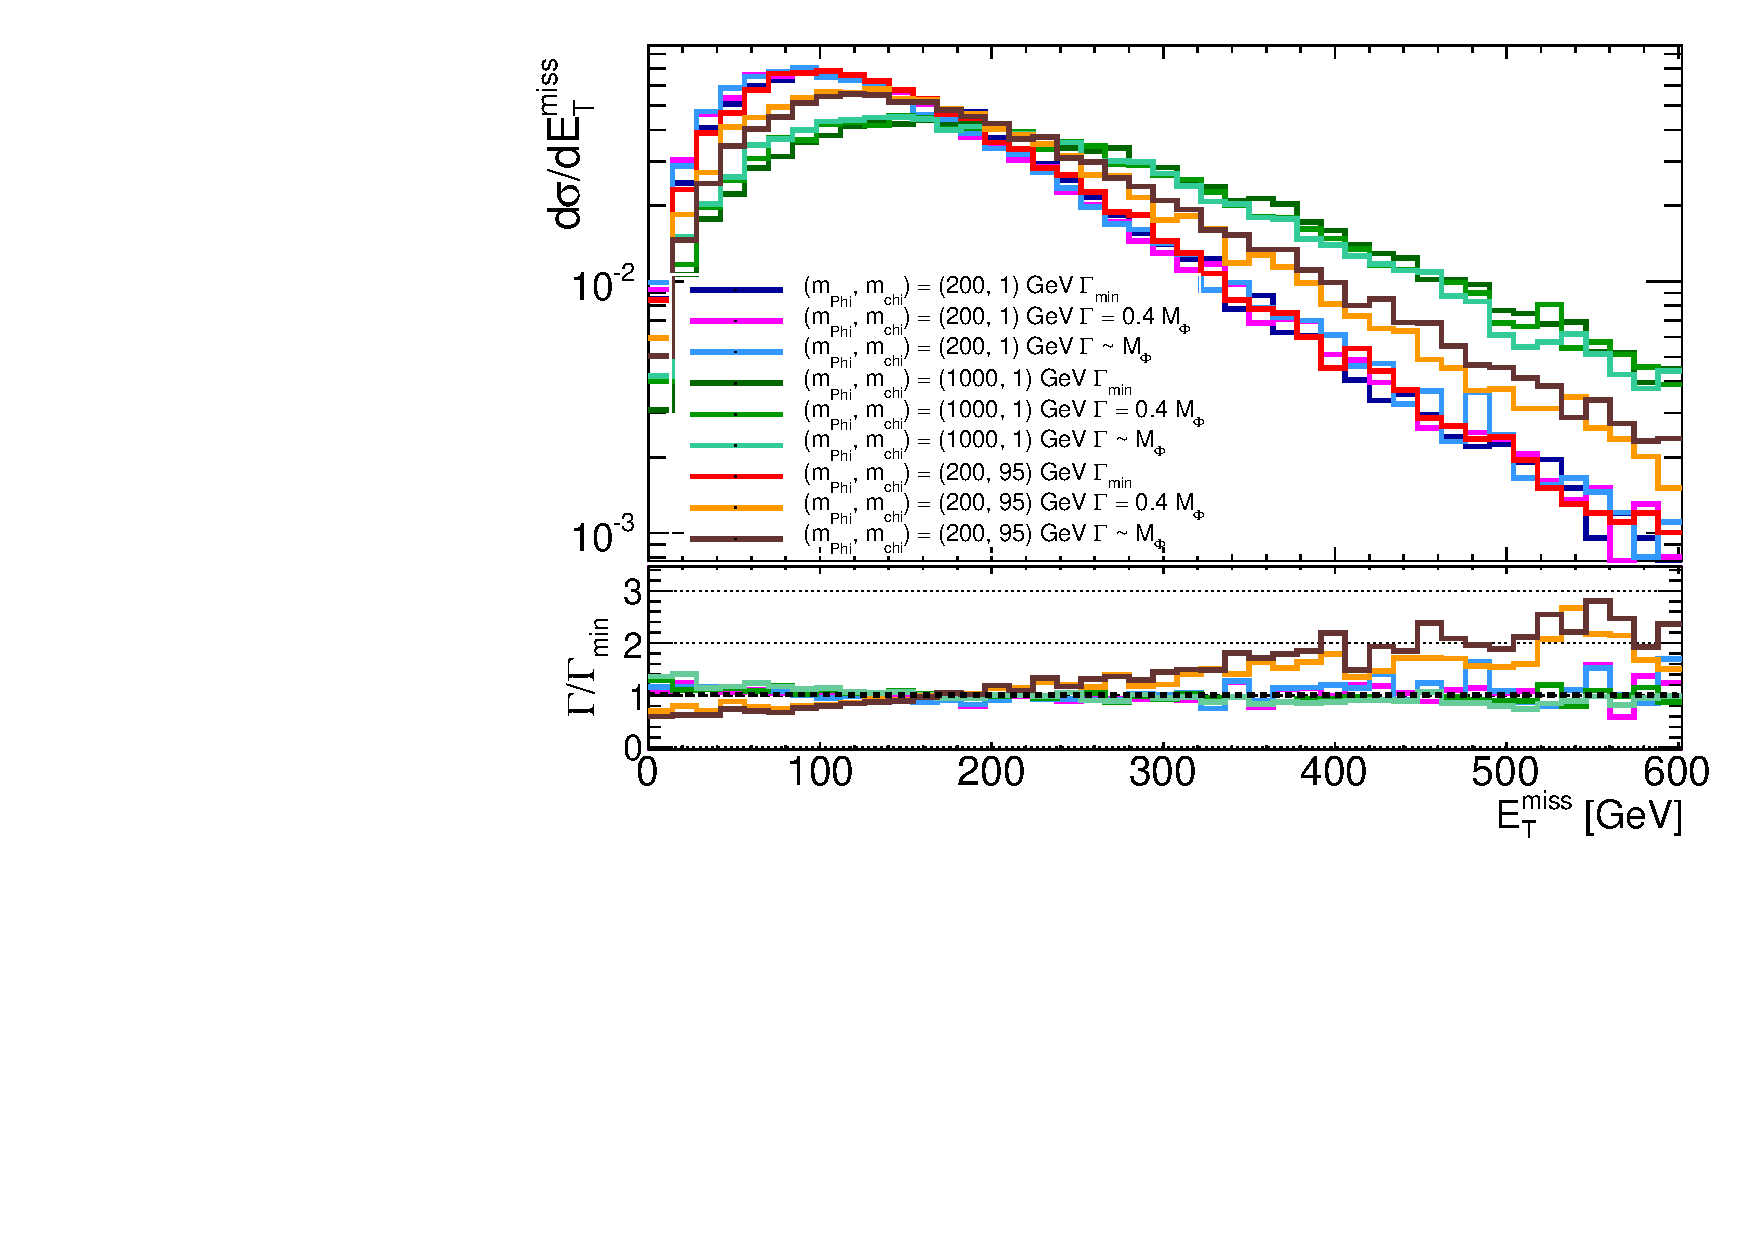
\includegraphics[width=0.95\textwidth]{figures/ttbar/ScalarWidth.pdf}
    \vspace{2mm}
    \caption{\label{fig:widthlargescan} Dependence of the kinematics on the width of a scalar mediator $t\bar{t}$+\MET{}. The width is increased up to the mediator mass. Choices of mediator and Dark Matter masses such that $m_{\phi,a}$ is slightly larger than $2m_\chi$ is the only case that shows a sizeable variation of the kinematics as a function of the width.  
    }
\end{center}
\end{figure}

The points for the parameter scan chosen for this model are listed in Table~\ref{tab:mDMmMedScan_SP}, chosen
to be harmonized with those for other analyses employing the same scalar model as benchmark. 
Based on the sensitivity considerations above, DM masses are only simulated up to 500 GeV (but the 5 TeV mediator point is retained)
leading to a total of 24 benchmark points. However for these searches we recommend to generate and simulate scalar and pseudoscalar
models separately, as the kinematics differs due to the different coupling of the mediator to the final state top quarks in the two cases,
as shown in Figs.~\ref{fig:scanPhi} and ~\ref{fig:scanPhiPseudo}.

Similar studies were performed in the $b \bar b$ case. It was found that they 
show the same weak dependence of the kinematics of the event on the mediator width.
The same benchmark parameters of the $t\bar t$ case could then be chosen.